\documentclass[9pt, compsoc, technote, a4paper]{IEEEtran}
\IEEEoverridecommandlockouts
% The preceding line is only needed to identify funding in the first footnote. If that is unneeded, please comment it out.
\usepackage{cite}
\usepackage{amsmath,amssymb,amsfonts}
\usepackage{algorithmic}
\usepackage{graphicx}
\usepackage{textcomp}
\usepackage{xcolor}
\usepackage{multirow}
\usepackage{lipsum}
\usepackage[colorlinks=true, urlcolor=blue, linkcolor=red]{hyperref}

\usepackage{pgfplots}
\pgfplotsset{width=0.47\textwidth,height=0.33\textwidth,compat=1.9}
% \usepgfplotslibrary{external}   % Externalizing the figures
% \tikzexternalize

\usepackage{float} % for [H] option
    
\begin{document}

% Author and Titling
\title{Political Fundraising Analysis in Washington State}

\author{\small{Dylan Kasanders}

}

\maketitle

\section{Introduction}
I work at my university doing data entry for our Advancement department. I am responsible for updating and maintaining records that are essential for fundraising and reaching out to donors. This hands-on experience exposed me to the intricate world of fundraising, and I became fascinated by the patterns and trends you were able to piece apart through donation records. Inspired by this, I wanted to take a look at fundraising patters for elections, specifically in Washington State.
\\
For this project I looked at Contributions to Candidates and Political Committees [1], a dataset published by the Washington State Open Data Portal. The dataset contained fundraising from election cycles 2007 to 2029. To narrow down the dataset, we will look at data between election years 2008 to 2024. The data originates from cash and in-kind contributions made to Washington state candidates and political candidates as reported to the PDC on forms C3, C4, and Schedule C.
\\
The two questions I aim to answer are the following:
\begin{enumerate}
    \item In a solid blue state, do Democrats continually outperform Republicans in fundraising?\\
    I hypothesise that Democrats do out fundraise Republicans, but Republicans are more incentivized to donate when the opposition is in power.
    \item In what areas do Democrats consistently outperform Republicans and vice versa?\\
    I hypothesise that Democrats cosistently outperform in statewide elections, while Republicans do better in local elections.
\end{enumerate}

\section{Analysis}
Looking at this dataset, there were various null values in certain fields that sparked alarm for further investigation. After looking into it further, the null values are due to that field not being applicable to that donation. For example, donations made to a particular party that weren't tied to a specific office election had the "office" attribute noted as null. The null values in the dataset seem to indicate that the respective attribute wasn't applicable to the source material or didn't apply to the nature of the donation rather than any necessary data being missing.
\\
Democrats consisently out fundraise Republicans in Washington state. Across the years, the Democrats have received 1,285,969 donations with an average donation amount of \$287.08. Republicans have received less donations with only 866,973 donations. However, on average the amount donated is greater than the Democrat average. Republican donations are on average \$316.38. Constructing a t-test to see if there is statistically significant difference between the average donation amounts of Democrats and Republicans, we get a t-value of -6.518 (with 2,152,940 degrees of freedom) decisively rejecting the null hypothesis of the sample means of both Republican and Democrat donation amounts being equal (p-value less than 0.00001).

\begin{figure}[H]
    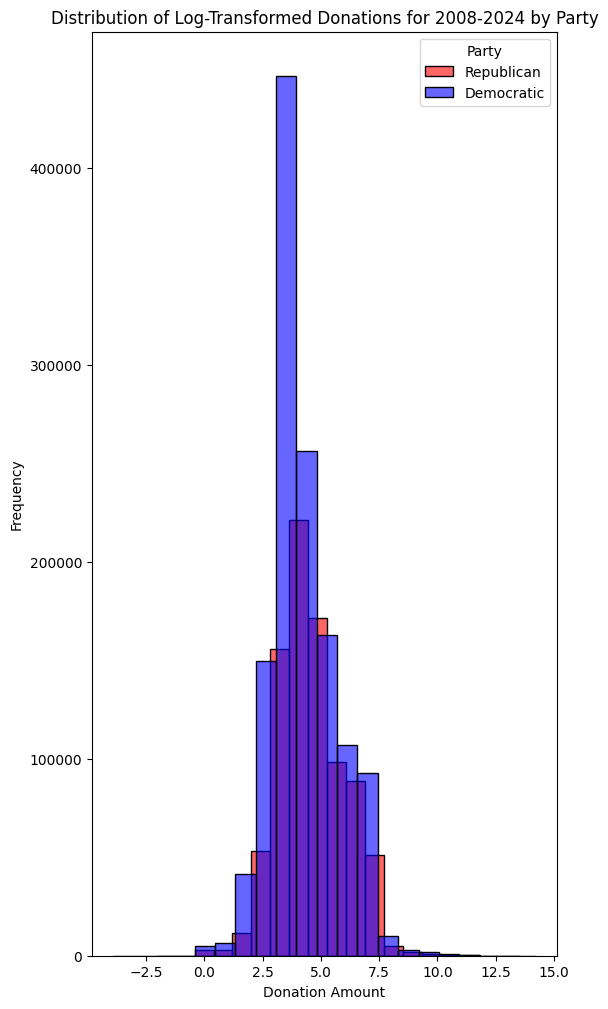
\includegraphics[width=1\linewidth]{2008-2024-party-hists.png}
\end{figure}
I looked at total donations per election year across both Republican and Democrats to see how donations for each party across the years. Adjusting for inflation, we construct the following graph with a regression line.
\begin{figure}[H]
    \begin{center}
        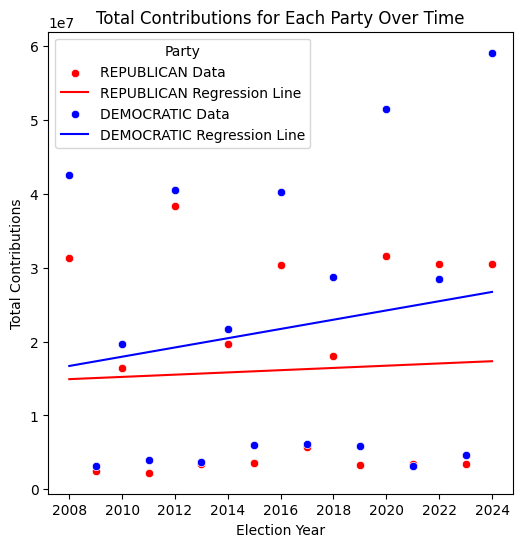
\includegraphics[width=0.8\linewidth]{regression-lines.png}
    \end{center}
\end{figure}
Democrats consistently raise more money compared to Republicans annually. Despite a positive coefficient for Democrat fundraising over time and a negative coefficient for Republicans, neither of the regressions proved statistically significant to indicate that the amount of fundraising either party gains is changing over the years.\\

\begin{figure}[H]
    \begin{center}
        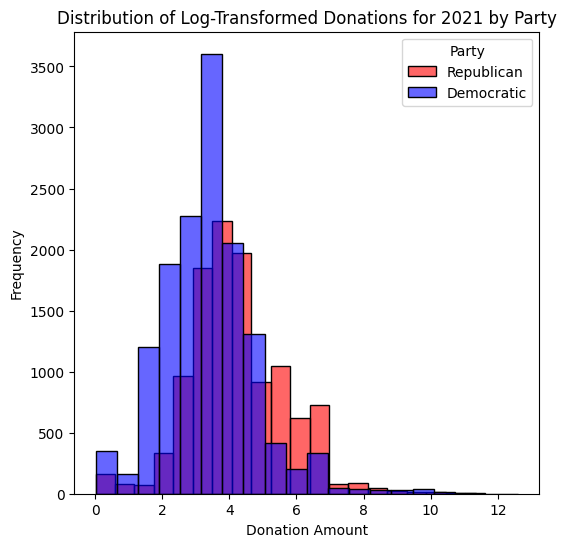
\includegraphics[width=1\linewidth]{2021-data.png}
        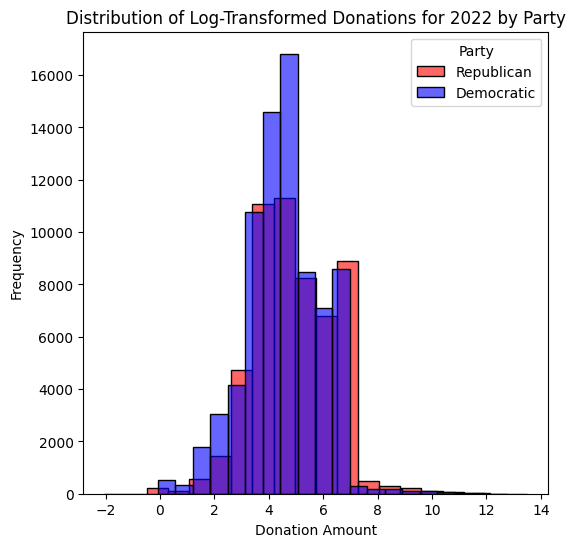
\includegraphics[width=1\linewidth]{2022-data.png}
    \end{center}
\end{figure}
    

The only times Republicans raised more money compared to Democrats was in 2021 and 2022, years when Democrats were in control of the Presidency. We notice despite in both of these years Democrats having more donations compared to Republicans, Republicans on average donated more compared to Republicans (mean of 306.61 to 222.59). Looking at histograms of donation amounts across both years, we observe that Republican donation amounts are more right-skewed to higher donation amounts, attributing to the higher mean donation amount
Republicans have compared to Democrats.\\
In 2021, Republican donation efforts were focused on a variety of County positions. For every county position, Republicans managed to 
out fundraise Democrats, with Democrats only donating for County Council Member Position 5. This was an election between Republican Sam Low and Democrat Brandy Donaghy.
This was an election that Republicans ultimately won with 60.59\% of the vote.\\
\begin{figure}[H]
    \begin{center}
        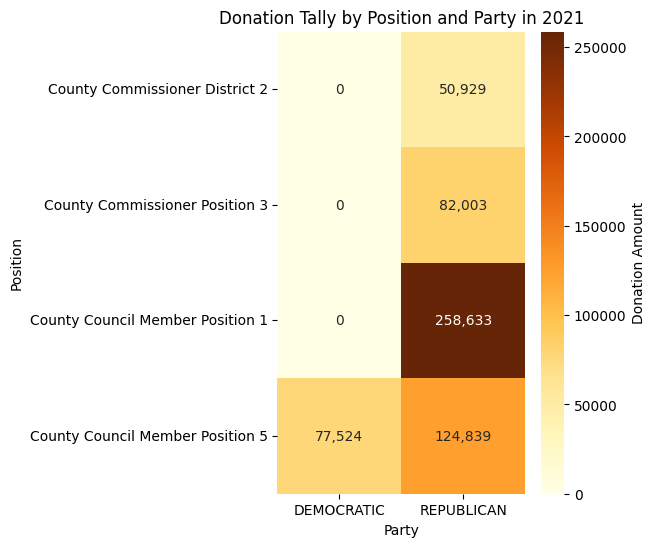
\includegraphics[width=1\linewidth]{donation-tally-2021.png}
    \end{center}
\end{figure}
In 2022 there's a similar trend. Democrats had more donations, but on average were less compared to Republicans. Fundraising was spent around State Representative positions, with Democrats raising \$10,327,785.30 for State Representative elections and Republicans raising \$10,034,664.10.\\
\begin{figure}[H]
    \begin{center}
        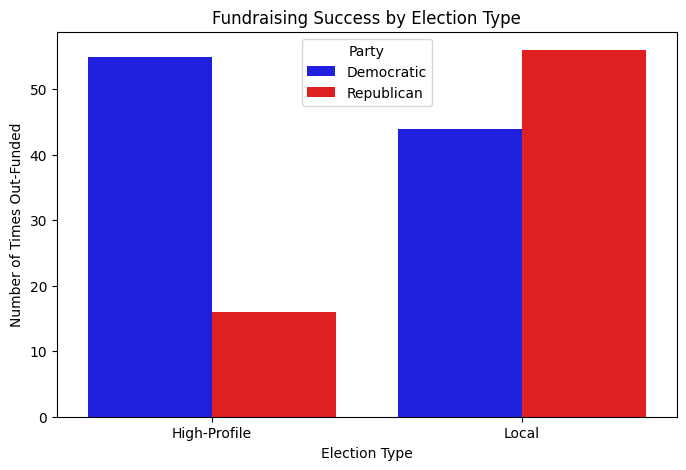
\includegraphics[width=1\linewidth]{fundraising-succ.png}
    \end{center}
\end{figure}
Democrats consistently outperform Republicans in high-profile offices, while Republicans do better in local elections. Looking at all of the donations tailored for a specific office, we can categorically split up the offices into two categories: high profile elections and low profile elections. High profile elections were defined as statewide and legislative offices that have impact at the state level. These include positions such as Governor, Attorney General, and Public Lands Commissioner. On the other hand, low profile elections refer to local offices, which primarily cover governmental power to a specific city or county. This includes positions such as Mayor, City Council Member, and School Director. Categorizing the offices by high profile and low profile allows us to look at the fundraising trends for Democrats and Republicans.\\


\section{Conclusion}
This dataset showcased that Democrats consistently out fundraise Republicans in Washington State, both in total donations and number of contributions. However, Republican donors tend to give larger individual donation amounts, and have our fundraising Democrats in the 2021 and 2022 election cycles. Additionally, while Democrats dominate fundraising for high-profile statewide elections, Republicans perform better in local races. Looking at the differences between how much Democrats fundraise on average compared to Republicans between these two election type categories, we see that Democrats on average out fundraise Republicans by roughly 1 million dollars for high-profile offices, while Republicans on average out fundraise Democrats by roughly \$29,000.

These insights could help to highlight the strategic differences in fundraising between the two parties. The Democratic party is able to rely on a broader state-wide level of support, and are able to get more low-dollar donations compared to the Republican party. On the other hand, Republican fundraising efforts appear to be more concentrated among high-dollar contributors, channeled into local elections. Understanding these patterns could inform future political fundraising strategies, and how to navigate political fundraising in a state with a solid tilt to one political party. 


\section{Source}
This dataset was sourced from the Washington State Open Data Portal. You can get the data \href{https://catalog.data.gov/dataset/contributions-to-candidates-and-political-committees}{here.}



\end{document}